% ======================= Pre-Amble =========================

\documentclass[11pt, oneside]{article}   	% use "amsart" instead of "article" for AMSLaTeX format 
                     						%imports package {article} and specify option(s) [11pt, oneside]
\usepackage{geometry}                		% See geometry.pdf to learn the layout options. There are lots.                                        

\geometry{letterpaper}                   		% ... or a4paper or a5paper or ... 
%\geometry{landscape}                		% Activate for rotated page geometry

\usepackage[parfill]{parskip}    		        % Activate to begin paragraphs with an empty line rather than an indent

\usepackage[hidelinks]{hyperref}                % Allows for clickable references

%American Mathematics Society packages
\usepackage{amsmath}	   %math
\usepackage{amssymb}       %symbols
\usepackage{amsthm}          %theorems

%Graphics
\usepackage{graphicx, subcaption}
\usepackage[usenames, dvipsnames]{color}     % font colour:    \textcolor{<colour>}{text}
      									%highlight text:  \colorbox{<color>}{text}
									
									%list of colours: https://www.sharelatex.com/learn/Using_colours_in_LaTeX

%Images		                
\graphicspath{ {images/} }                          %directory that your images are located in within your current directory
	

%Footnote Spacing
\setlength{\footnotesep}{0.4cm}                  %specify spacing b/w footnotes
\setlength{\skip\footins}{0.6cm}                    % space b/w footnotes and textbody

%Table
\usepackage[none]{hyphenat}                    % Stops breaking-up words in a table (i.e. no hyphens)                                                             

\usepackage{array}   
\newcolumntype{x}[1]{>{\centering\let\newline\\\arraybackslash\hspace{0pt}}p{#1}}       %center fixed column width: x{<len>}                      
\newcolumntype{$}{>{\global\let\currentrowstyle\relax}}                                                   % let us apply things (e.g. bold/italicize) to entire row            
\newcolumntype{^}{>{\currentrowstyle}}
\newcommand{\rowstyle}[1]{\gdef\currentrowstyle{#1} #1\ignorespaces}

%Bibliography
\usepackage[numbers,sort&compress]{natbib}   %for multiple references: sorts  (i.e. [1,2] NOT [2, 1] )
                                           				  %                                     compresses (i.e. [1-3] )
\usepackage[nottoc]{tocbibind}                            %add bibliography to table of contents

%Bullets
\usepackage{enumerate}     %specify type of enumeration: \being{enumerate}[<type of enumeration>]

%QED
\newcommand*{\QEDA}{\hfill\ensuremath{\blacksquare}}         %make qed filled square:    \QEDA
%\newcommand*{\QEDB}{\hfill\ensuremath{\square}}               %make qed empty square: \QEDB 

%Header and Footer
\usepackage{fancyhdr}
\usepackage{lastpage}      %ensures you can reference LastPage (i.e. Page 2 of 10)

%Diagrams
\usepackage[latin1]{inputenc}
\usepackage{tikz}
\usepackage{tkz-berge}
\usetikzlibrary{shapes,arrows}

%Miscellaneous
\usepackage{dirtytalk}    %quotations: use \say  

\usepackage{caption}
\captionsetup[figure]{labelfont=bf}    %make figure labels boldface
\captionsetup[table]{labelfont=bf}     %make table labels boldface


%=========== Header & Footer =========================

\pagestyle{fancy}
\lhead{Stephanie Knill} 		% controls the left corner of the header
\chead{} 					% controls the center of the header
\rhead{} 					% controls the right corner of the header
\lfoot{} 					% controls the left corner of the footer
\cfoot{Page~\thepage\ of \pageref{LastPage}} 				% controls the center of the footer
												%Page~\thepage\  if just want Page x
\rfoot{}			 		% controls the right corner of the footer
\renewcommand{\headrulewidth}{0.4pt}
\renewcommand{\footrulewidth}{0.4pt}

\setlength{\headsep}{0.3in}		%space b/w page header and body

% ======================== Document ======================
\begin{document}

\title{MATH 442 --- Assignment 3 \\
\line(1,0){360} \\              %(slope x, y){length of line}
}
\author{
Stephanie Knill \\
54882113 \\
Due: January 21, 2015}

\date{}                   % Activate:  display a given date (e.g. {August 4} ) or no date (empty {} )
                                    %No activate: display current date
\maketitle


\thispagestyle{empty}                   %Remove header from this (first) page. Change empty -> plain to keep numbering

% ================= Questions ================

\section*{Question 13}

{\textbf{Proof 1:} We will show that, in any graph the sum of the degrees of all vertices is even.

Let $G$ be a graph with edges $n \in \{0\} \cup \mathbb{N}$.
Since every edge joins 2 vertices, the sum of the degrees of all vertices for $n$ edges is $2n$. By the definition of even, $2n$ is even, thus proving that in any graph the sum of the degrees of all vertices is even. \QEDA

{\textbf{Deduction 1:} in any graph, there exists an even number of vertices of odd degree.

\textit{Proof by Contradiction:}
 Assume that in a graph there is an \textit{odd} number of vertices of odd degree. Since the sum of even vertices is always even, let us only examine the vertices of odd degree. Summating an odd number of odd vertices gives us an odd sum of degrees. However from above we know that the sum of all degrees is even. Therefore we have arrived at a contradiction and our initial assumption is false. We can then conclude that in any graph, there exists an even number of vertices of odd degree. \QEDA

{\textbf{Proof 2:} We will prove by contradiction that, if I am at a party and have shaken hands with 5 people, then there exists someone else at the party that has shaken hands with an odd number of people.

\textit{Proof by Contradiction:}
Let the graph $G$ be a graph with nodes as people at the party and an edge joining two nodes if those two people have shaken hands. From Proof 1, we know that the sum of the degrees of all vertices is even. Since the vertex representing myself is of degree 5 and there is an even number of vertices of odd degree by Deduction 1, then there must exist at least 1 other vertex of odd degree. \QEDA


\cleardoublepage
\section*{Question 14}

The graph $G$ of $n$ vertices has edge set $E(G)$ with regular degree of $r$. Its complement $\overline{G}$ of $n$ vertices  with regular degree $r$ has the edge set $E(K_n) - E(G)$. In a regular complete graph $K_n$, the number of degrees at each vertex is $n-1$. Therefore for a graph with $n$ vertices of degree $r$, its complement graph $\overline{G}$ has $n$ vertices of regular degree given by
\begin{align*}
\overline{r} & = (\text{number of edges } E(K_n)) - (\text{number of edges } E(G)) \\
& = n-1-r \\
\end{align*}



\section*{Question 15}

{\textbf{Proof:} We will show that, if a graph $G$ is self-complementary then $G$ has $4k$ or $4k+1$ vertices, where $k \in \mathbb{Z}$.

Since $G$ is self-complementary, the number of edges in $\overline{G}$ is equal to the number of edges in $G$. This can be expressed as
$$(\text{number of edges } E(K_n)) - (\text{number of edges } E(G)) = (\text{number of edges } E(G))$$
For a graph $G$ of $n$ vertices, let its edge set $E(G)$ have $x$ edges and the edge set of the complete graph $E(K_n)$ have $\frac{n(n-1)}{2}$ edges. Thus we can rewrite it as
\begin{align*}
\frac{n(n-1)}{2} - x  & = x\\
\frac{n(n-1)}{2} & = 2x \\
\frac{n(n-1)}{4} & = x \in \mathbb{Z}
\end{align*}


Since $\frac{n(n-1)}{4} \in \mathbb{Z}$, we have two cases: $4 \mid n$ and $4 \mid (n -1)$. In the first case, we have the number of vertices to be
$$n = 4k, \quad k \in \mathbb{Z}$$

While in the second case 
\begin{align*}
n -1 & = 4k \\
n & = 4k + 1, \quad k \in \mathbb{Z}
\end{align*}

Combining both cases, we have that if $G$ is a self-complementary graph, then $G$ has $4k$ or $4k+1$ vertices, $k \in \mathbb{Z}$. \QEDA
\cleardoublepage
	
To find a self-complementary graph of 8 vertices, let us first start with any smaller self-complementary graph that is easily found. Without loss of generality, we will use the self-complementary graph $G$ of 4 vertices (Figure~\ref{4 nodes}) as it was discussed in class.

\begin{figure}[h]
%Latex Documentation: http://www.texample.net/tikz/examples/tkz-berge/
\centering

\begin{tikzpicture}[scale=0.75,transform shape]
  \Vertex[x=0,y=0]{4}
  \Vertex[x=0,y=2]{1}
  \Vertex[x=2,y=0]{2}
  \Vertex[x=2,y=2]{3}

  \tikzstyle{LabelStyle}=[fill=white,sloped]
  %Edges bend left
  \tikzstyle{EdgeStyle}=[bend left]		%\Edge[label=$120$](A)(B)  %if want to label the edge
      			
  %Edges bend right
  \tikzstyle{EdgeStyle}=[bend right]

  %Edges straight
  \tikzstyle{EdgeStyle}=[]
      \Edge(1)(3)
      \Edge(1)(4)
      \Edge(4)(2)    
\end{tikzpicture}

\caption{Self-complementary graph $G$ of 4 vertices}
\label{4 nodes}
\end{figure}

Now, we will add to our self-complementary graph a path $P_4$ which consists of 4 vertices $v_1, v_2, v_3,$ and $v_4$. Here we will join vertex $v_2$ and $v_3$ to every vertex of $G$. The resulting self-complementary graph of 8 vertices is depicted in Figure~\ref{8 nodes}.

\begin{figure}[h]
%Latex Documentation: http://www.texample.net/tikz/examples/tkz-berge/
\centering
\begin{tikzpicture}[scale=0.75,transform shape]
  \Vertex[x=0,y=0]{4}
  \Vertex[x=0,y=2]{1}
  \Vertex[x=2,y=0]{2}
  \Vertex[x=2,y=2]{3}
  \Vertex[L = $v_1$, x=6,y=4]{v1}
  \Vertex[L = $v_2$, x=6,y=2]{v2}
  \Vertex[L = $v_3$, x=6,y=0]{v3}
  \Vertex[L = $v_4$, x=6,y=-2]{v4}

  \tikzstyle{LabelStyle}=[fill=white,sloped]	

  %Edges straight
  \tikzstyle{EdgeStyle}=[]			%\Edge[label=$120$](A)(B)  %if want to label the edge
      \Edge(1)(3)
      \Edge(1)(4)
      \Edge(4)(2)   
      \Edge(v1)(v2)
      \Edge(v2)(v3)
      \Edge(v3)(v4)
      
  %Edges straight + colour
  \tikzstyle{EdgeStyle}=[red]
  	\Edge(v2)(3)
	\Edge(v2)(2)
	\Edge(v2)(4)
	\Edge(v3)(3)
	\Edge(v3)(2)
	\Edge(v3)(1)
  %Edges bend right
  \tikzstyle{EdgeStyle}=[bend right, red]
  	\Edge(v2)(1)
    
  %Edges bend left
  \tikzstyle{EdgeStyle}=[bend left, red]	
  	\Edge(v3)(4)
  
\end{tikzpicture}

\caption{Self-complementary graph of 8 vertices}
\label{8 nodes}
\end{figure}

\section*{Question 16}

\textbf{Proof:} We will show that, if a self-complementary graph has $4n+1$ vertices then one of the vertices has degree at least $2n$.

%Let the edge set of a graph $G$ be $E(G)$ and the edge set of its complementary graph $\overline{G}$ be $E(K_n) - E(G)$. 
Let $G$ be a self-complementary graph of $4n+1$ vertices.
From Question 15, we know that if a graph $G$ is self-complementary, then the number of edges in its complement $\overline{G}$ is equal to the number of edges in $G$. Thus the degree of each corresponding vertex pair in $G$ and $\overline{G}$ must summate to the number of degrees in its complete graph. By definition, the complete graph $K_{4n+1}$.
has $4n$ degrees for each vertex.

Since $G$ is self-complementary, $G$ and $\overline{G}$ are isomorphic---if we can show that for each corresponding vertex pair $v_i$ and $\overline{v_i}$ of $G$ and $\overline{G}$ respectively, either $v_i$ or $\overline{v_i}$ is of degree at least $2n$, then we are done. The set of possible degrees for each corresponding vertex pair can be broken into 3 cases:

\begin{itemize}
\item \textbf{Case 1:} $deg(v_i) = 2n$. Since $deg(v_i) + deg(\overline{v_i}) = 4n$, then $deg(\overline{v_i}) = 2n$.
\item \textbf{Case 2:} $deg(v_i) > 2n$. Since $deg(v_i) + deg(\overline{v_i}) = 4n$, then $deg(\overline{v_i}) < 2n$.
\item \textbf{Case 3:} $deg(v_i) < 2n$. Since $deg(v_i) + deg(\overline{v_i}) = 4n$, then $deg(\overline{v_i}) > 2n$.
\end{itemize}

%\textbf{Case 1:} $deg(v_i) = 2n$
%
%Since $deg(v_i) + deg(\overline{v_i}) = 4n$, then $deg(\overline{v_i}) = 2n$.
%
%\textbf{Case 2:} $deg(v_i) > 2n$					%\hspace{1cm} 
%
%Since $deg(v_i) + deg(\overline{v_i}) = 4n$, then $deg(\overline{v_i}) < 2n$.
%
%\textbf{Case 3:} $deg(v_i) < 2n$
%
%Since $deg(v_i) + deg(\overline{v_i}) = 4n$, then $deg(\overline{v_i}) > 2n$.

In each of the three cases, there existed a vertex in $G$ or $\overline{G}$ that had a degree of at least $2n$. \QEDA

\section*{Question 17}
For each of the following graphs (Figure~\ref{isomorphism}), each have 5 vertices and 6 edges. However, only graphs (a) and (f) are isomorphic.

\begin{figure}[h]
%Latex Documentation: http://www.texample.net/tikz/examples/tkz-berge/
\centering

\begin{subfigure}[b]{0.25\columnwidth}             
\centering
  \begin{tikzpicture}[scale=0.75,transform shape]
  	\Vertex[x=0,y=0]{D}
 	\Vertex[x=0,y=2]{A}
 	\Vertex[x=2,y=0]{C}
 	\Vertex[x=2,y=2]{B}
  	\Vertex[x=1,y=1]{E}
  	%\Vertex[L = $v_1$, x=6,y=4]{v1}

  \tikzstyle{LabelStyle}=[fill=white,sloped]	
  %Edges straight
  \tikzstyle{EdgeStyle}=[]			%\Edge[label=$120$](A)(B)  %if want to label the edge
	\Edge(A)(B)
	\Edge(B)(C)
	\Edge(C)(D)
	\Edge(D)(A)
	\Edge(A)(E)
	\Edge(E)(B)
  \end{tikzpicture}
  \caption{}
  \label{A}
\end{subfigure}
\begin{subfigure}[b]{0.25\columnwidth}
  \centering
  \begin{tikzpicture}[scale=0.75,transform shape]
  	\Vertex[x=0,y=0]{D}
 	\Vertex[x=0,y=2]{A}
 	\Vertex[x=2,y=0]{C}
  	\Vertex[x=2,y=2]{B}
  	\Vertex[x=1,y=1]{E}
  	%\Vertex[L = $v_1$, x=6,y=4]{v1}

 	 \tikzstyle{LabelStyle}=[fill=white,sloped]	

  	%Edges straight
 	 \tikzstyle{EdgeStyle}=[]			%\Edge[label=$120$](A)(B)  %if want to label the edge
		\Edge(A)(B)
		\Edge(B)(C)
		\Edge(C)(D)
		\Edge(D)(A)
		\Edge(A)(E)
		\Edge(E)(C)
  \end{tikzpicture}
  \caption{}
\end{subfigure}
\begin{subfigure}[b]{0.25\columnwidth}
  \centering
  \begin{tikzpicture}[scale=0.75,transform shape]
	\Vertex[x=0,y=0]{D}
	\Vertex[x=0,y=2]{A}
	\Vertex[x=2,y=0]{C}
	\Vertex[x=2,y=2]{B}
	\Vertex[x=1,y=1]{E}
		 %\Vertex[L = $v_1$, x=6,y=4]{v1}

	\tikzstyle{LabelStyle}=[fill=white,sloped]	

	%Edges straight
	\tikzstyle{EdgeStyle}=[]			%\Edge[label=$120$](A)(B)  %if want to label the edge
		\Edge(A)(B)
		\Edge(B)(E)
		\Edge(E)(C)
		\Edge(E)(D)
		\Edge(A)(D)
		\Edge(A)(E)
	\end{tikzpicture}
	\caption{}
\end{subfigure}
\begin{subfigure}[b]{0.25\columnwidth}
  \centering
    \begin{tikzpicture}[scale=0.75,transform shape]
      \Vertex[x=0,y=0]{D}
      \Vertex[x=0,y=2]{A}
      \Vertex[x=2,y=0]{C}
      \Vertex[x=2,y=2]{B}
      \Vertex[x=1,y=1]{E}
      %\Vertex[L = $v_1$, x=6,y=4]{v1}
    
      \tikzstyle{LabelStyle}=[fill=white,sloped]	
    
      %Edges straight
      \tikzstyle{EdgeStyle}=[]			%\Edge[label=$120$](A)(B)  %if want to label the edge
    	\Edge(A)(B)
    	\Edge(B)(C)
    	\Edge(D)(A)
    	\Edge(A)(E)
    	\Edge(E)(B)
    	\Edge(E)(D)
    \end{tikzpicture}
    \caption{}
\end{subfigure}
\begin{subfigure}[b]{0.25\columnwidth}
  \centering
    \begin{tikzpicture}[scale=0.75,transform shape]
      \Vertex[x=0,y=0]{D}
      \Vertex[x=0,y=2]{A}
      \Vertex[x=2,y=0]{C}
      \Vertex[x=2,y=2]{B}
      \Vertex[x=1,y=1]{E}
      %\Vertex[L = $v_1$, x=6,y=4]{v1}
    
      \tikzstyle{LabelStyle}=[fill=white,sloped]	
    
      %Edges straight
      \tikzstyle{EdgeStyle}=[]			%\Edge[label=$120$](A)(B)  %if want to label the edge
    	\Edge(B)(C)
    	\Edge(D)(A)
    	\Edge(A)(E)
    	\Edge(E)(B)
    	\Edge(E)(D)
    	\Edge(E)(C)
    \end{tikzpicture}
    \caption{}
\end{subfigure}
\begin{subfigure}[b]{0.25\columnwidth}
  \centering
    \begin{tikzpicture}[scale=0.75,transform shape]
      \Vertex[x=0,y=0]{d}
      \Vertex[x=0,y=2]{a}
      \Vertex[x=2,y=0]{c}
      \Vertex[x=2,y=2]{b}
      \Vertex[x=1,y=1]{e}
      %\Vertex[L = $v_1$, x=6,y=4]{v1}
    
      \tikzstyle{LabelStyle}=[fill=white,sloped]	
    
      %Edges straight
      \tikzstyle{EdgeStyle}=[]			%\Edge[label=$120$](A)(B)  %if want to label the edge
    	\Edge(A)(B)
    	\Edge(B)(C)
    	\Edge(D)(A)
    	\Edge(E)(B)
    	\Edge(E)(D)
    	\Edge(E)(C)
    \end{tikzpicture}
    \caption{}
\end{subfigure}


\caption{Graphs of 5 vertices and 6 edges with varying connectivity.}
\label{isomorphism}
\end{figure}

Let us first examine graphs (c) and (e), as they are the only graphs with a vertex of degree 4. Here, both graphs have $deg(E)=4$. Unfortunately, vertex $E$ of graph (c) connects to a vertex $C$ of degree 1, whereas vertex $E$ of graph (e) only connects to vertices of degree 2. Thus, we can eliminate these two graphs.

Of the remaining four graphs, only graph (d) has a node of degree 1; this can similarly be eliminated.

Now focussing our attention to just graphs (a), (b), and (f), we notice that all graphs have two vertices of degree 3 and three vertices of degree 2. In graphs (a) and (f) the degree 3 vertices are connected by an edge---this is not the case in graph (b), however. With graph (b) now eliminated, we can see that an isomorphism $\psi$ exists between graphs (a) and (f):
\begin{align*}
\psi: \; A & \rightarrow e \\
B & \rightarrow b \\
C & \rightarrow a \\
D & \rightarrow d \\
E & \rightarrow c \\
\end{align*} 

\section*{Question 18}

\textbf{Number of vertices of $Q_k$}

By definition, a $k$-cube graph $Q_k$ is a graph whose vertices correspond to the sequences ($a_1, a_2, \ldots, a_k$), where each $a=0$ or 1, and whose edges join those sequences that differ in just one place. Thus we can express the number of vertices in $Q_k$ as a permutation of 2 choices (0 or 1) over a set of size $k$:
$$\text{Number of vertices } Q_k = 2^k$$  \QEDA

\textbf{Number of edges of $Q_k$}

By the definition of $Q_k$, we have $k$ possible sequences that differ by 1 place, which represents the number of edges emerging from each vertex. Since there are $2^k$ vertices, we have $2^k \cdot k$ edges emerging from the vertices of $Q_k$. But since each edge has 2 ends, we have counted each edges twice. Hence, the number of edges of $Q_k$ is given by
$$\text{Number of edges } Q_k = \frac{2^k \cdot k}{2} = 2^{k-1} \cdot k$$ \QEDA









\end{document} 